\documentclass{article}


\usepackage[final]{neurips}
\usepackage[utf8]{inputenc} % allow utf-8 input
\usepackage[T1]{fontenc}    % use 8-bit T1 fonts
\usepackage{hyperref}       % hyperlinks
\usepackage{url}            % simple URL typesetting
\usepackage{booktabs}       % professional-quality tables
\usepackage{amsfonts}       % blackboard math symbols
\usepackage{nicefrac}       % compact symbols for 1/2, etc.
\usepackage{microtype}      % microtypography
\usepackage{graphicx}
\usepackage{subcaption}
\usepackage{wrapfig}
\usepackage{float}
\usepackage{ragged2e}
\usepackage{amsmath}
\usepackage{mathtools}
\usepackage{booktabs}
\usepackage{caption}
\usepackage{float}
\usepackage{titlesec}
\usepackage{capt-of}
\usepackage{array}
\usepackage{arydshln}
\usepackage{xepersian}
\settextfont{XB Yas.ttf}
\setlength\dashlinedash{0.2pt}
\setlength\dashlinegap{1.5pt}
\setlength\arrayrulewidth{0.3pt}

%Widows & Orphans & Penalties

\widowpenalty500
\clubpenalty500
\clubpenalty=9996
\exhyphenpenalty=50 %for line-breaking at an explicit hyphen
\brokenpenalty=4991
\predisplaypenalty=10000
\postdisplaypenalty=1549
\displaywidowpenalty=1602
\floatingpenalty = 20000

\title{پرسش و پاسخ تصویری در فارسی}

\author{%
  مریم سادات هاشمی \\
  دانشکده مهندسی کامپیوتر\\
  دانشگاه علم و صنعت ایران\\
  \texttt{m\_hashemi94@cs.iust.ac.ir} \\
   \And
    علیرضا اصغری \\
   دانشکده مهندسی کامپیوتر\\
   دانشگاه علم و صنعت ایران\\
    \texttt{a\_asghari@comp.iust.ac.ir}
}


\begin{document}


\begin{minipage}{0.1\textwidth}% adapt widths of minipages to your needs

\includegraphics[width=1.1cm]{iust_logo.png}
\end{minipage}%
\hfill%
\begin{minipage}{0.9\textwidth}\raggedleft
دانشگاه علم و صنعت ایران\\
یادگیری عمیق (بهار ۱۳۹۹)\\
\end{minipage}


\makepertitle

\begin{abstract}
	در سال‌های اخیر پیشرفت‌های زیادی در مسائل هوش مصنوعی و یادگیری عمیق که در تقاطع دو حوزه پردازش زبان طبیعی و بینایی ماشین قرار می‌گیرند؛ رخ داده است. یکی از مسائلی که اخیرا مورد توجه قرارگرفته است؛ پرسش و پاسخ تصویری است. با توجه به یک تصویر و یک سؤال به زبان طبیعی، سیستم سعی می‌کند با استفاده از عناصر بصری تصویر و استنتاج جمع‌آوری شده از سوال متنی، پاسخ صحیح را پیدا کند. هدف ما در این پروژه ...
\end{abstract}
\section{مقدمه}
 لورم ایپسوم متن ساختگی با تولید سادگی نامفهوم از صنعت چاپ و با استفاده از طراحان گرافیک است. چاپگرها و متون بلکه روزنامه و مجله در ستون و سطرآنچنان که لازم است و برای شرایط فعلی تکنولوژی مورد نیاز و کاربردهای متنوع با هدف بهبود ابزارهای کاربردی می باشد.

\section{کار‌های مرتبط / پیش‌زمینه}
لورم ایپسوم متن ساختگی با تولید سادگی نامفهوم از صنعت چاپ و با استفاده از طراحان گرافیک است. چاپگرها و متون بلکه روزنامه و مجله در ستون و سطرآنچنان که لازم است و برای شرایط فعلی تکنولوژی مورد نیاز و کاربردهای متنوع با هدف بهبود ابزارهای کاربردی می باشد.

\section{مدل پیشنهاد شده}
{
	در این بخش ابتدا نحوه‌ی آماده‌سازی مجموعه‌داده را توضیح می‌دهیم و سپس به شرح روش‌های پیاده‌سازی شده در این پروژه می‌پردازیم.
	
	\subsection{تهیه‌ی مجموعه‌داده}
	{
		مجموعه‌داده‌ای که برای حل این مسئله انتخاب کردیم؛ مجموعه داده
		 \href{https://visualqa.org/vqa_v1_download.html}{\lr{VQA v1}} 
		 است. مشخصات کامل مجموعه داده را می‌توانید در جدول 1 مشاهده کنید.
		 \begin{table}
			 \begin{center}
			 	\begin{tabular}{ c c c c } 
			 		\hline
			 		& \textbf{تعداد تصاویر} & \textbf{تعدادسوالات} & \textbf{تعداد پاسخ‌ها} \\
			 		\hline \hline
			 		\textbf{داده‌های آموزشی} & 82,783 & 248,349 &  2,483,490 \\
					
					\textbf{داده‌های ارزیابی} & 40,504 & 121,512 & 1,215,120 \\
					
					\textbf{داده‌های تست} & 81,434 & 244,302 & \\
					\hline
			 	\end{tabular}
			 \end{center}
		 \caption{مشخصات مجموعه‌داده VQA}
	 	\end{table}
		برای ترجمه مجموعه‌داده از دو ابزار Google‌ و ترگمان استفاده کردیم. در این مجموعه‌داده برای هر تصویر سه سوال وچود دارد و برای هر سوال 10 پاسخ موجود می‌باشد. در این مجموعه‌داده سه نوع سوال وجود دارد. نوع اول بله و خیر است. نوع دوم تعداد یک شی در تصویر است و نوع سوم مربوط به سوالات دیگر است. توزیع طول سوالات و پاسخ‌ها و 30 پاسخ پرتکرار در این مجموعه‌داده را برای دو حالت ترجمه Google‌‌ و ترگمان را در شکل های 
		\ref{fig:9}
		،
		\ref{fig:10}
		و 
		\ref{fig:11}
		می‌توانید مشاهده کنید. 
	}
	\subsection{\lr{LSTM Q + norm I} \cite{antol2015vqa}}
	{
		\begin{figure}
			\centering
			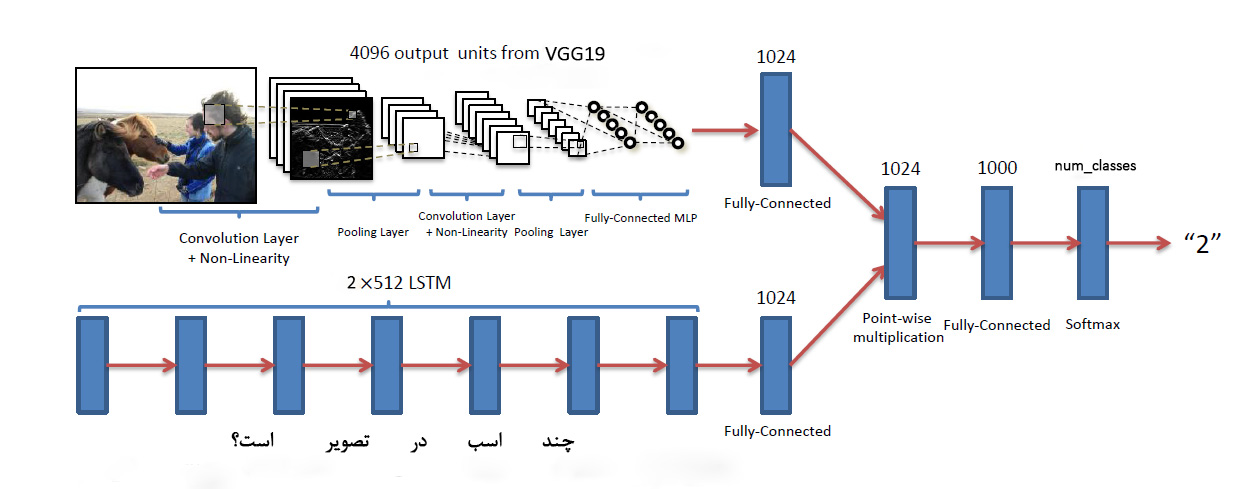
\includegraphics[scale=0.4]{images/Vanilla_Network.jpg}
			\caption{ساختار کلی روش \lr{LSTM Q + norm I}  .}
			\label{fig:3}
		\end{figure}
		این روش ساده‌ترین روش یادگیری عمیق برای حل مسئله پرسش و پاسخ تصویری است. در اینجا مسئله VQA به عنوان یک مسئله طبقه‌بندی در نظر گرفته می‌شود که در آن 1000 پاسخ پرتکرار به عنوان کلاس‌ها انتخاب می‌شوند.  ساختار کلی این شبکه در شکل 
		\ref{fig:3}
		نشان داده شده است. ابتدا با عبور دادن تصاویر از شبکه 
		\lr{VGG19}
		 برای هر تصویر یک بردار ویژگی 4096تایی در لایه‌ی ماقبل آخر در شبکه‌ی
		  \lr{VGG19}
		   تولید می‌شود. از طرفی دیگر با عبور سوال‌ها از لایه‌یEembedding برای هر کلمه موجود در سوال یک بردار 300تایی تولید می‌شود. سپس از طریق 2 لایه LSTM بردار ویژگی معنایی سوال استخراج  می‌شود. هر یک از بردارهای ویژگی تصویر و سوال را به یک لایه‌ی Dense  1024 واحدی می‌دهیم تا ابعاد بردار‌ها مشابه هم شوند. برای ترکیب بردار ویژگی سوال و تصویر از ضرب نقطه‌ای استفاده می‌کنیم. از این بردار ترکیب شده به عنوان ورودی برای لایه‌ی کاملا متصل استفاده می‌کنیم و در نهایت با عبور از یک لایه softmax کلاس(پاسخ) پیش‌بینی شده بدست می‌آید.
	}

	\subsection{\lr{Stacked Attention Network} \cite{yang2016stacked} }
	{
		ایده‌ی اصلی روش SAN‌ این است که ابتدا از سوال، یک  بازنمایی معنایی و مفهومی استخراج می‌کند. سپس از آن به عنوان یک کوئری برای پیدا کردن مناطقی از تصویر که مرتبط با سوال است؛ استفاده می‌کند. غالباً در مسئله VQA نیاز است تا چندین مرحله استدلال صورت بگیرد. بنابراین در این شبکه از چندین لایه برای جستجو در تصویر استفاده می‌کنیم تا به تدریج به جواب مورد نظر برسیم. ساختار کلی شبکه SAN را در شکل 
		\ref{fig:1}
		می‌توانید مشاهده کنید. شبکه SAN از سه جز اصلی تشکیل شده است: 1) مدل تصویر که با استفاده از CNN ویژگی‌های سطح بالایی را از تصویر استخراج می‌کند. 2) مدل سوال که با استفاده از CNN یا LSTM ویژگی‌های معنایی سوال را استخراج می‌کند. 3) مدل
		 \lr{stacked attention}
		 ‌ که از طریق استدلال چند مرحله‌ای مناطقی از تصویر که مرتبط به سوال است را پیدا می‌کند تا پاسخ را پیش‌بینی کند.
		\begin{figure}
			\centering
			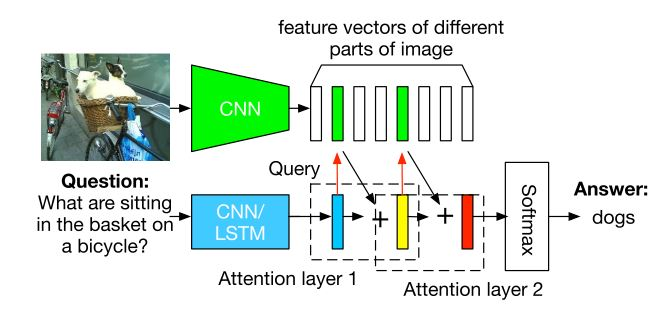
\includegraphics[scale=0.5]{images/san.jpg}
			\caption{ساختار کلی روش SAN .}
			\label{fig:1}
		\end{figure}
	
		\subsubsection{مدل تصویر}
		{
			در این بخش برای استخراج ویژگی از شبکه‌ی
			 \lr{VGG16}
			 ‌ استفاده می‌کنیم و ویژگی‌ها را از آخرین لایه‌ی
			 \lr{pooling}
			  ‌شبکه بدست می‌آوریم. ابتدا تمام تصاویر را به
			 \lr{448×448}
			  تغییر سایز می‌دهیم و بعد از این که تابع پیش‌پردازش موجود برای شبکه‌ی 
			 \lr{VGG16}
			   را بر روی تصاویر اعمال کردیم، تصاویر را برای استخراج ویژگی به شبکه می‌دهیم. بنابراین برای هر تصویر یک ویژگی با ابعاد
			 \lr{512×14×14}
			 حاصل می‌شود. در حقیقت، برای هر تصویر به تعداد
			 \lr{14×14}
			 منطقه استخراج می‌شود که هر منطقه به وسیله‌ی یک بردار ویژگی 512تایی بازنمایی می‌شود. برای راحتی، از یک لایه‌ی
			 \lr{Dense}
			 بعد از شبکه‌ی 
			 \lr{VGG16}
			استفاده می‌کنیم تا ابعاد بردار ویژگی مناطق مشابه با ابعاد بردار ویژگی سوال شود.
		}
	
		\subsubsection{مدل سوال}
		{
			\begin{figure}
				\centering
				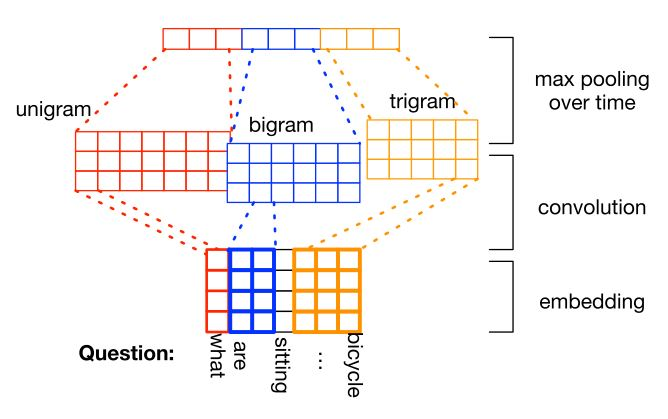
\includegraphics[scale=0.5]{images/san_cnn.jpg}
				\caption{مدل سوال براساس CNN .}
				\label{fig:2}
			\end{figure}
			برای استخراج ویژگی‌های معنایی از سوال، از هر دو روش  LSTM‌ و CNN یک بعدی استفاده می‌کنیم. در هر دو روش ابتدا سوال را به یک دنباله‌ی عددی تبدیل می‌کنیم و سپس این دنباله‌ها را به یک لایه‌ی Embedding‌ می‌دهیم. در روش
			 LSTM
			خروجی لایه Embedding را به دو لایه‌ی LSTM می‌دهیم و خروجی آخرین لایه‌ی مخفی LSTM را به عنوان بردار ویژگی سوال در نظر می‌گیریم. در روش CNN خروجی Embedding را به سه لایه‌ی کانولوشنی یک بعدی با فیلترهایی با سایز 1، 2، 3 می‌دهیم که به ترتیب ترکیب‌های یک کلمه‌ای ، دو کلمه‌ای و سه کلمه‌ای را برای ما استخراج می‌کند. در نهایت بر روی خروجی هر سه لایه تابع maxpooling  را اعمال می‌کنیم و با قرار دادن این سه خروجی در کنار هم بردار ویژگی سوال بدست می‌آید. شکل 
			\ref{fig:2}
			مدل سوال بر اساس CNN را نشان می‌دهد.
		}
	
		\subsubsection{مدل \lr{stacked attention}}
		{
			در این بخش، مدل
			\lr{stacked attention}
			 با توجه به ماتریس ویژگی تصویر و بردار ویژگی سوال پاسخ را از طریق استدلال چند مرحله‌ای پیش‌بینی می‌کند. در بسیاری  از موارد، یک پاسخ فقط مربوط به یک ناحیه کوچک از تصویر است. بنابراین، استفاده از یک ماتریس ویژگی کلی  برای تصویر می‌تواند به دلیل وجود نویزهای مناطق بی‌ربط  به پاسخ، منجر به نتایج نامطلوبی شود. در عوض، استدلال از طریق چندین لایه توجه، قادر است به تدریج مناطق غیرمرتبط با جواب را فیلتر کند و از ماتریس ویژگی تصویر حذف کند. بدین منظور ماتریس ویژگی تصویر
		 $v_I$
	    و بردار ویژگی سوال
	    $v_Q$
	    ، را به یک لایه Dense می‌دهیم و خروجی این لایه را به یک تابع softmax می‌دهیم تا توزیع توجه را بر روی نواحی تصویر بدست آوریم. بنابراین داریم:
	    \begin{equation}
	    	h_A = tanh (W_{I,A} v_I \oplus (W_{Q,A}v_Q + b_A))
	    \end{equation}
	    \begin{equation}
	    	p_I = softmax(W_Ph_A + b_P)
	    \end{equation}
	    
	    بر اساس توزیع توجه
	     $p_i$
	     ، جمع وزن‌دار بردارهای تصویر را که هر کدام متناظر به یک منطقه هست را محاسبه می‌کنیم. سپس
	     $\tilde{v}_I$
	      را با بردار ویژگی سوال ترکیب می‌کنیم و یک کوئری برای لایه‌ی بعدی توجه ایجاد می‌کنیم.	    
	     \begin{equation}
	      	\tilde{v}_I =\sum_i p_iv_i,
	     \end{equation}
	     \begin{equation}
	        u =\tilde{v}_I + v_Q.
	     \end{equation}
	      این روش را به تعداد k بار تکرار می‌کنیم. در نهایت از u در لایه‌ی k برای پیش‌بینی پاسخ استفاده می‌کنیم:
	     \begin{equation}
	     	p_{ans} =softmax(W_uu^K + b_u)
	     \end{equation}
	     
		}
	}

	\subsection{\lr{HieCoAttention} \cite{lu2016hierarchical}}
	{
		\begin{figure}
			\centering
			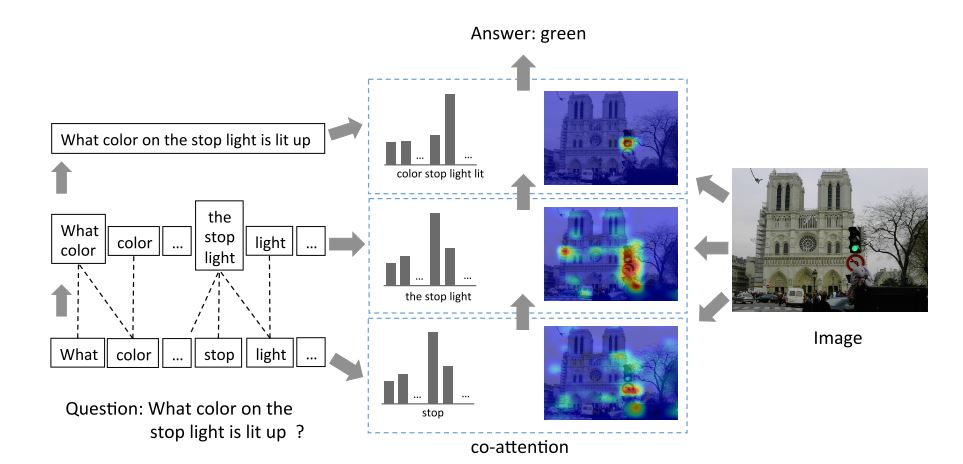
\includegraphics[scale=0.6]{images/hiecoattention.JPG}
			\caption{ساختار کلی روش HieCoAttention}
			\label{fig:7}
		\end{figure}
		روش پیشنهاد شده در 
		\cite{}
		دارای دو ویژگی مهم است. ویژگی اول بازنمایی سلسله‌مراتبی سوال و ویژگی دوم مکانیزم coattention می‌باشد. در ادامه این دو خصوصیات را شرح می‌دهیم.
		
		\subsubsection{بازنمایی سلسله‌مراتبی سوال}
		{
			\begin{figure}
				\centering
				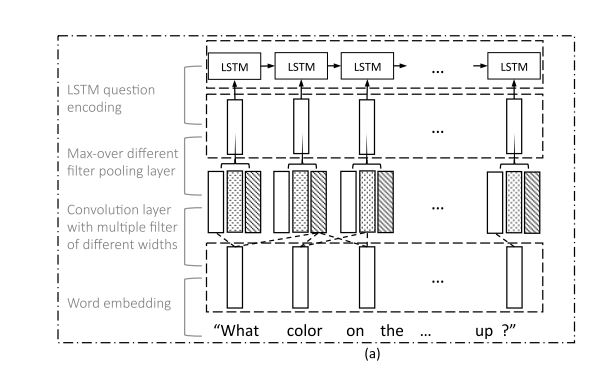
\includegraphics[scale=0.5]{images/hierarchical.jpg}
				\caption{بازنمایی سلسله‌مراتبی سوال.}
				\label{fig:4}
			\end{figure}
		
			در این بخش برای هر سوال سه سطح Embedding را محاسبه می‌کنیم. اولین Embedding مربوط به کلمات است که بعد از این‌که سوال را به دنباله‌های عددی تبدیل کردیم؛ با عبور دادن این دنباله‌ها از لایه‌ی Embedding ، بردارهای Embedding‌ کلمات بدست می‌آید. برای محاسبه سطح بعدی Embedding که مربوط به عبارات است از کانولوشن‌های یک بعدی با فیلترهایی با سایز 1، 2 و 3 استفاده می‌کنیم و سپس با اعمال تابع Maxpooling بردار Embedding هر عبارت بوجود می‌آید. در نهایت از Embedding عبارات  برای محاسبه‌ی Embedding  کل سوال استفاده می‌کنیم. این کار توسط یک لایه LSTM انجام می‌شود. بنابراین  برای هر سوال به صورت سلسله‌مراتبی سه سطح Embedding کلمه، عبارت و سوال تولید می‌شود. بازنمایی سلسله‌مراتبی سوال در شکل
			\ref{fig:4}
			 به تصویر کشیده شده است.
		}
		\subsubsection{مکانیزم coattention}
		{
			\begin{figure}
				\centering
				\begin{subfigure}[b]{0.4\textwidth}
					\centering
					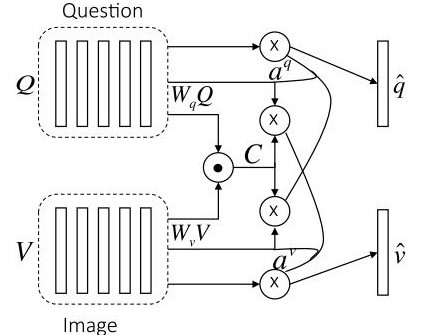
\includegraphics[width=0.85\linewidth]{images/parallel.JPG}
					\caption{}
				\end{subfigure}%
				\begin{subfigure}[b]{0.42\textwidth}
					\centering
					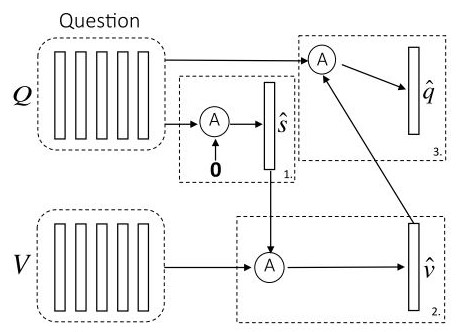
\includegraphics[width=0.85\linewidth]{images/alternating.JPG}
					\caption{}
				\end{subfigure}%
				\caption
				{
					(آ) 
					\lr{parallel coattention}
					(ب)
					\lr{alternating coattention}
				}
				\label{fig:5}
			\end{figure}
			در 
			\cite{}
			 دو مکانیزم برای coattention پیشنهاد شده است که از نظر ترتیب تولید 
			\lr{attention map}
			 برای سوال و تصویر با هم تفاوت دارند. اولین مکانیزم که
			\lr{parallel coattention}
			 نامیده می‌شود، باعث تولید attention به طور همزمان برای سوال و تصویر می‌شود. به مکانیزم دوم
			\lr{alternating coattention}
			 می‌گویند که برای تولید attention‌ برای سوال و تصویر به صورت تناوبی عمل می‌کند (شکل 
			\ref{fig:5}
			 ). این مکانیزم coattention در هر سه سطح سلسله‌مراتبی سؤال اجرا می‌شوند.  در این پروژه ما از مکانیزم 
			 \lr{parallel coattention}
			 استفاده می‌کنیم. در این مکانیزم با محاسبه شباهت بین ویژگی‌های تصویر و سوال، تصویر و سؤال را به هم متصل می‌کنیم. اگر بردار ویژگی تصویر را با V و بازنمایی سوال را با Q نشان دهیم؛ ماتریس شباهت C 
			 به صورت زیر محاسبه می‌شود:
			 \begin{equation}
			 	C = tanh(Q^TW_bV)
			 \end{equation}
			 
			 پس از محاسبه ماتریس شباهت، برای محاسبه بردار وزن‌های attention برای تصویر و سوال از روابط زیر استفاده می‌کنیم:
			 \begin{equation}
			 \begin{aligned}
			 	H^v = tanh(W_vV + (W_qQ)C), \ \ \ \ \  H^q = tanh(W_qQ+ (W_vV)CT)\\
			 	a^v = softmax(w^T_{hv}H^v), \ \ \ \ \  a^q = softmax(w^T_{hq}H^q) \ \ \ \ \ \ \ \ \ \ \ \ \ 
			 \end{aligned}
			 \label{eq:1}
			 \end{equation}
			 که در عبارت 
			 \ref{eq:1}
			 $W_v$
			 ، 
			 $W_q$
			 ،
			 $w_{hv}$
			 و
			 $w_{hq}$
			 پارامترهای وزن هستند. 
			 $a_v$
			 و 
			 $a_q$
			 نیز به ترتیب وزن‌های attention برای تصویر و سوال هستند. با توجه به وزن‌های attention ، بردارهای توجه تصویر و سوال به وسیله‌ی جمع وزن‌دار ویژگی‌های تصویر و ویژگی‌های سوال با وزن‌های attention محاسبه می‌شوند:
			 \begin{equation}
			 \hat{v} =\sum_{n+1}^{N} a^v_nv_n,\ \ \ \ \ \hat{q} = \sum_{t=1}^{T}a^q_t q_t
			 \end{equation}
			 
		}
	
		\subsubsection{پیش‌بینی پاسخ}
		{
			\begin{figure}
				\centering
				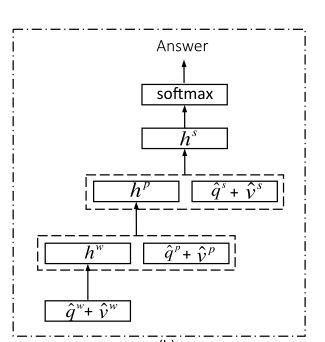
\includegraphics[scale=0.6]{images/answer.JPG}
				\caption{پیش‌بینی پاسخ}
				\label{fig:6}
			\end{figure}
		
			ما پاسخ را بر اساس coattention تصویر و سوال بدست آمده در هر سه سطح Embedding پیش‌بینی می‌کنیم. از یک پرسپترون چندلایه (MLP) استفاده می‌کنیم تا ویژگی‌های attention را همان طور که در شکل 
		\ref{fig:6}	
			نشان داده شده است؛ ترکیب کنیم.
			\begin{equation}
			\begin{aligned}
			h^w = tanh(W_w(\hat{q}^w + \hat{v}^w))\ \ \ \  \\
			h^p = tanh(W_p[\hat{q}^p + \hat{v}^p), h^w]) \\
			h^s = tanh(W_s[(\hat{q}^s + \hat{v}^s), h^p]) \\
			p = softmax(W_hh^s)  \ \ \ \ \ \ \ \ \ \ \ \ \ 
			\end{aligned}
			\end{equation}
		
			 $W_W$
			 ، 
			 $W_p$
			 ،
			 $W_s$
			  و
			 $W_h$
			  	پارامترهای وزن هستند. p احتمال پاسخ نهایی است.
		}
	}

}


\section{نتایج}
{	
	\subsection{\lr{LSTM Q + norm I}}
	{
		\begin{table}[H]\centering
			\begin{latin}
				\begin{small}
					\begin{tabular}{ c|| c c c c || c c c c} \toprule
						\multicolumn{1}{c ||}{ }&\multicolumn{4}{c||}{\textbf{Google Translation}} & \multicolumn{4}{c}{\textbf{Targoman Translation}} \\ \midrule
						\textbf{Method} & \textbf{yes/no} & \textbf{Number} & \textbf{Other} & \textbf{All} & \textbf{yes/no} & \textbf{Number} & \textbf{Other} & \textbf{All} \\ \midrule
						\textbf{lstm Q + VGG19} & 76.14\ & 32.97\ & 35.78\ & 50.53\ & 75.58\ & 32.61\ & 33.53\ & 49.15\ \\
						%\textbf{lstm Q + VGG19} & \ & \ & \ & \ & \ & \ & \ & \ \\
						\bottomrule
					\end{tabular}
				\end{small}
			\end{latin}
			\caption{}
		\end{table}
	
		\begin{table}[H]\centering
			\begin{latin}
				\begin{small}
					\begin{tabular}{ c|| c c c c || c c c c} \toprule
						\multicolumn{1}{c ||}{ }&\multicolumn{4}{c||}{\textbf{ٍEnglish-paperToken}} & \multicolumn{4}{c}{\textbf{English-kerasToken}} \\ \midrule
						\textbf{Method} & \textbf{yes/no} & \textbf{Number} & \textbf{Other} & \textbf{All} & \textbf{yes/no} & \textbf{Number} & \textbf{Other} & \textbf{All} \\ \midrule
						\textbf{lstm Q + VGG19} & 78.43\ & 33.7\ & 37.99\ & 52.58\ & 78.53\ & 31.91\ & 38.78\ & 52.79\ \\
						\bottomrule
					\end{tabular}
				\end{small}
			\end{latin}
			\caption{}
		\end{table}
	
		\begin{table}[H]\centering
			\begin{latin}
				\begin{small}
					\begin{tabular}{ c|| c c c c } \toprule
						\multicolumn{1}{c ||}{ }&\multicolumn{4}{c}{\textbf{Google Translation}}  \\ \midrule
						\textbf{Method} & \textbf{yes/no} & \textbf{Number} & \textbf{Other} & \textbf{All} \\ \midrule
						\textbf{BilstmQ+resNet152} & 76.46\ & 31.63\ & 38.6\ & 51.89\ \\
						\textbf{lstmQ+resNet152} & 76.83\ & 31.75\ & 38.77\ & 52.13\ \\ 
						\textbf{CNNQ+resNet152} & 78.34\ & 31.91\ & 38.98\ & 52.82\ \\
						\bottomrule
					\end{tabular}
				\end{small}
			\end{latin}
			\caption{}
		\end{table}
	
	}
	\subsection{\lr{Stacked Attention Network}}
	{
		\begin{table}[H]\centering
			\begin{latin}
				\begin{small}
					\begin{tabular}{ c|| c c c c || c c c c} \toprule
						\multicolumn{1}{c ||}{ }&\multicolumn{4}{c||}{\textbf{Google Translation}} & \multicolumn{4}{c}{\textbf{Targoman Translation}} \\ \midrule
						\textbf{Method} & \textbf{yes/no} & \textbf{Number} & \textbf{Other} & \textbf{All} & \textbf{yes/no} & \textbf{Number} & \textbf{Other} & \textbf{All} \\ \midrule
						\textbf{SAN\_LSTM\_2} & 77.83\ & 33.19\ & 39.08\ & 52.84\ & 75.95\ & 31.61\ & 36.82\ & 50.81\ \\ 
						\textbf{SAN\_CNN\_2} & 77.49\ & 33.17\ & 39.18\ & 52.76\ & 76.48\ & 32.29\ & 37.37\ & 51.37\ \\
						\bottomrule
					\end{tabular}
				\end{small}
			\end{latin}
			\caption{}
		\end{table}
		
		\begin{table}[H]\centering
			\begin{latin}
				\begin{small}
					\begin{tabular}{ c|| c c c c } \toprule
						\multicolumn{1}{c ||}{ }&\multicolumn{4}{c}{\textbf{Google Translation}}  \\ \midrule
						\textbf{Method} & \textbf{yes/no} & \textbf{Number} & \textbf{Other} & \textbf{All} \\ \midrule
						\textbf{SAN\_LSTM\_1} & 77.46\ & 32.23\ & 38.35\ & 52.22\ \\
						\textbf{SAN\_LSTM\_2} & 77.83\ & 33.19\ & 39.08\ & 52.84\ \\ 
						\textbf{SAN\_LSTM\_3} & 77.12\ & 32.56\ & 38.62\ & 52.27\ \\
						\bottomrule
					\end{tabular}
				\end{small}
			\end{latin}
			\caption{}
		\end{table}
	
	}
	\subsection{\lr{HieCoAttention}}
	{
		\begin{table}[H]\centering
			\begin{latin}
				\begin{small}
					\begin{tabular}{ c|| c c c c || c c c c} \toprule
						\multicolumn{1}{c ||}{ }&\multicolumn{4}{c||}{\textbf{Google Translation}} & \multicolumn{4}{c}{\textbf{Targoman Translation}} \\ \midrule
						\textbf{Method} & \textbf{yes/no} & \textbf{Number} & \textbf{Other} & \textbf{All} & \textbf{yes/no} & \textbf{Number} & \textbf{Other} & \textbf{All} \\ \midrule
						\textbf{CoAttention} & 76.62\ & 32.7\ & 38.12\ & 51.85\ & 74.18\ & 32.41\ & 32.47\ & 48.07\ \\ 
						\bottomrule
					\end{tabular}
				\end{small}
			\end{latin}
			\caption{}
		\end{table}
		
	}
	

	


}
\section{تحلیل}
لورم ایپسوم متن ساختگی با تولید سادگی نامفهوم از صنعت چاپ و با استفاده از طراحان گرافیک است. چاپگرها و متون بلکه روزنامه و مجله در ستون و سطرآنچنان که لازم است و برای شرایط فعلی تکنولوژی مورد نیاز و کاربردهای متنوع با هدف بهبود ابزارهای کاربردی می باشد.


\section*{مراجع}
\LTR
\begin{latin}
	\bibliographystyle{abbrv}
	\bibliography{bibliography}
\end{latin}


\end{document}
